\section{Evaluation}
\label{sec:eval}
The evaluation follows the objection path a comparison paper would face.  Do coarse public vocabularies create denominator errors?  Are counts grounded by witnesses rather than names?  Do source, probe, feature, and engine stresses preserve a finite kernel without becoming population claims?  Are projection-audit stages cheap enough to rerun when the denominator changes?  The schema, projections, source manifest, source-admission codebook, and retained-field universe are frozen before counting; exhaustive retained-field search is reported as a certificate check, while layer and placement are architecture-derived dimensions.  Execution is a post-freeze SQL-denominator consistency check: it validates probes but never admits rules or chooses fields; a non-interference check verifies that DuckDB/PostgreSQL validation files are not consumed by collision tables.  The table column ``Coll.'' is contract-level: a declared vocabulary collapses unequal public optimizer-contract signatures before any latency, plan-quality, or cost claim is interpreted.

The comparison surfaces are executable projection vocabularies and controls, not DBMS bug finders such as SQLancer~\cite{rigger2020sqlancer}, NoREC~\cite{rigger2020norec}, or other SQL fuzzing tools.  Those tools test execution behavior under generated oracles; OptSem-C audits whether a public comparison vocabulary has already collapsed unequal contracts.  Across the 26 public source surfaces, all expose keyword-style or operator-family labels, twelve expose yes/no-style controls, and none exposes the complete reference contract payload.  Reference comparison is the negative control, one-field projections are diagnostic ablations, and strengthened projections restore fields to localize missing information.  All projections are fixed before witness counting and evaluated over the same source-linked maps.  The question is how many witnesses are lost if equality is decided at that vocabulary, not whether every cited study made that exact projection.

\textbf{Coarse comparison induces concentrated, separable collisions.} The main empirical result is a finite counterexample to two coarse optimizer-comparison vocabularies, plus a positive result about narrower controls.  Table~\ref{tab:contract-collision} keeps public vocabularies, controls, stress rows, and separating fields on the same scale: keyword declares 2,284 equivalences and collapses 254 unequal reference signatures, while operator-only declares 2,268 and collapses 238.  These 11.1\% and 10.5\% fractions condition on equivalences declared by the tested vocabularies inside this corpus, not on optimizer papers.  The 492 primary records are concentrated: keyword records are BigQuery--ClickHouse (203), BigQuery--Trino (45), and ClickHouse--Trino (6); operator-only records are ClickHouse--Trino (123) and Spark SQL--Trino (115).  The remaining 17 engine pairs have zero headline collisions, so coarse labels often suffice for local-engine or non-boundary comparisons in this denominator.  The risk signal appears at cloud service, connector, distributed execution, and runtime-adaptation boundaries where public layer and placement distinctions carry the comparison.  The yes/no public-control view declares 2,036 equivalences but collapses only six, all in ClickHouse--Trino, a narrow positive result for enablement-style controls.  Primary collision pairs have reference-signature Jaccard distance 1.0 and differ by 9.09 and 5.84 evidence atoms on average.  The strict reference and strengthened surface controls have zero collapsed pairs; one-field stress rows show that a single optimizer dimension can make the denominator worse rather than safer.

\begin{table}[H]
\centering
\caption{Projection-induced contract-collision summary. Eq. is declared-equivalent engine--probe pairs; False is pairs whose exact public-contract signatures differ; Cond. is False/Eq.; Repair is the minimum separating field set.}
\label{tab:contract-collision}
\small
\begin{tabular}{lrrrl}
\toprule
Projection & Eq. & False & Cond. & Repair field(s) \\
\midrule
Keyword & 2,284 & 254 & 11.1\% & placement \\
Yes/No & 2,036 & 6 & 0.3\% & layer \\
Operator-only & 2,268 & 238 & 10.5\% & layer \\
\bottomrule
\end{tabular}
\Description{Summary table of projection-induced contract-collision counts and repair fields for keyword, yes/no, and operator-only projections.}
\end{table}


Representative witness audits appeared earlier in Table~\ref{tab:cases}; the evaluation now asks whether those examples are isolated or part of a finite kernel.

Table~\ref{tab:projection-surface-portfolio} brings the 26-row public-surface catalog into the paper.  It reports source documents that admit comparison vocabularies, not how often researchers use them.  Every admitted source exposes keyword or operator-family labels, twelve expose yes/no controls, and none exposes the full reference-signature payload.  PostgreSQL and Trino contribute 27.9\% and 21.3\% of admitted rules, while DuckDB and Snowflake contribute 7.3\% and 9.1\%; source-rich engines can create more measured opportunities, so pair counts are corpus-specific evidence rather than documentation-normalized prevalence.  If a comparison falls outside this finite catalog, the safe action is to rerun extraction rather than transfer the certificate.

\begin{table*}[t]
\centering
\caption{Projection-family synthesis over the fixed comparison set.  False-pair counts are lower-better: bold marks zero-collision controls or repairs, and underlining marks the largest unsafe family.}
\label{tab:baseline-portfolio}
\footnotesize
\setlength{\tabcolsep}{3pt}
\begin{tabular}{@{}p{2.45cm}p{3.00cm}rp{3.00cm}p{5.35cm}@{}}
\toprule
Family & Rows represented & Worst false pairs$\downarrow$ & Strongest check & Takeaway \\
\midrule
Reference controls & Exact; semantic surface & \textbf{0} & Same 88,536 comparisons & Exact equality preserves the denominator. \\
\addlinespace[1pt]
Public-label vocabularies & Keyword; yes/no; op-only & 254 & Wilson, bootstrap, leave-one-source & Public labels can be semantically unsafe. \\
\addlinespace[1pt]
One-field stress tests & Placement-only; state-only & 23,593 & Exhaustive finite audit & Single fields are not conservative. \\
\addlinespace[1pt]
Repair basis & Keyword: placement; op-only: layer; all: layer+placement & \textbf{0} & Counter-witnesses plus held-out repairs & Layer and placement resolve headline witnesses. \\
\addlinespace[1pt]
Resolution frontier & 256 subsets; 128 no-variant & \underline{59,546} & 14 minimal safe; 8 maximal unsafe & Safety is a finite frontier. \\
\bottomrule
\end{tabular}
\Description{Synthesis table grouping the projection audit into reference controls, public-label vocabularies, one-field stress tests, repair basis checks, and retained-field frontier checks.}
\end{table*}


Finite resampling keeps keyword at roughly 10--12\% and operator labels at roughly 9--12\% of corpus-specific declared equivalences.  Single-source removal is stricter to read: removing one source can delete original witnesses and create new ones, so the audit reports both nonzero counts and witness-identity movement rather than treating leave-one-source as population sampling.  The diagnosis column localizes the missing semantics: placement separates keyword, layer separates the operator row, and the strengthened semantic surface returns to zero collapsed pairs.  The sparse yes/no row is a positive boundary result for enablement-style controls: its six witnesses are all ClickHouse--Trino records and it is not used to claim broad binary-control risk.

\textbf{Projection kernels are measurable objects.} Figure~\ref{fig:projection-information} reports the finite information profile.  Reference signatures form 1,288 observed classes.  Keyword projection compresses them into 148 projected classes, retains 64\% of empirical signature entropy, and inflates declared equivalence by 12.5\%; operator-only retains more entropy but still leaves 238 pairwise collisions.  Placement-only and state-only surfaces show the opposite failure mode: a single field creates very large kernels.  The strengthened surface still has projected collisions at the signature-class level, but no pairwise collision over the engine-probe comparison set.

\begin{figure}[t]
\centering
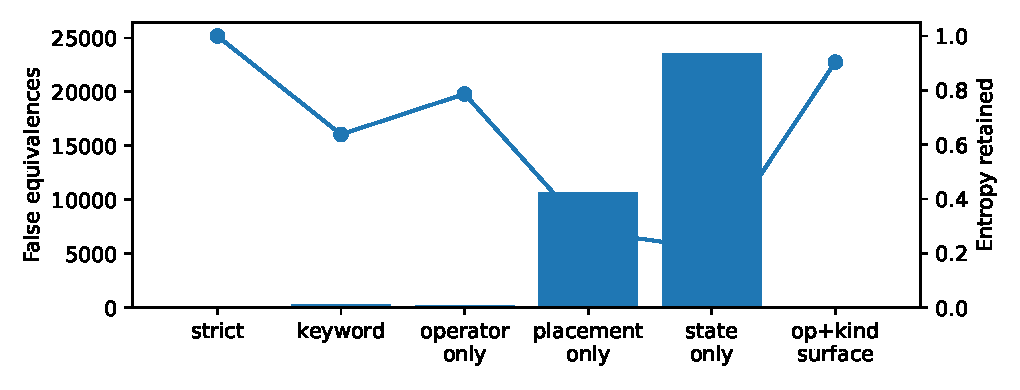
\includegraphics[width=\columnwidth]{figures/fig_projection_information.pdf}
\caption{Projection information profile. Bars show false equivalences induced by representative projections; the line shows empirical signature entropy retained by the projection.}
\Description{A bar and line chart comparing representative projections. Strict has zero false equivalences and entropy one; coarse projections lose entropy and introduce false equivalences.}
\label{fig:projection-information}
\end{figure}


\textbf{Resolution lattice stress test.}  Table~\ref{tab:resolution-lattice} enumerates all 256 retained-field subsets over the same 88,536 engine--probe comparisons.  The empty vocabulary declares 59,546 unsupported equivalences, and every singleton semantic field remains unsafe: operator leaves 238 collisions, kind 252, layer 449, and placement 10,702.  Excluding action-variant identifiers, the semantic lattice has 128 subsets, 44 unsafe regions, minimum safe field count two, 14 minimal safe vocabularies, and eight maximal unsafe vocabularies.  Ten concrete engine--probe witnesses cover all unsafe retained-field regions.

\begin{table}[t]
\centering
\caption{Exhaustive field-resolution lattice. Rows retain only the listed public optimizer fields. $|R|$ is retained fields; Classes is projected signature classes; Ent. is normalized entropy; Eq. is declared-equivalent pairs; False is unequal exact pairs still collapsed. Good rows drive False to zero with small $|R|$.}
\label{tab:resolution-lattice}
\footnotesize
\setlength{\tabcolsep}{2.5pt}
\begin{tabular}{@{}lrrrrr@{}}
\toprule
Fields & $|R|$ & Classes & Ent. & Eq. & False \\
\midrule
None & 0 & 1 & -0.000 & 61,576 & 59,546 \\
Operator & 1 & 387 & 0.787 & 2,268 & 238 \\
Action kind & 1 & 183 & 0.661 & 2,282 & 252 \\
Layer & 1 & 52 & 0.552 & 2,479 & 449 \\
Placement & 1 & 9 & 0.280 & 12,732 & 10,702 \\
Operator+layer & 2 & 591 & 0.850 & 2,030 & 0 \\
Kind+placement & 2 & 214 & 0.680 & 2,030 & 0 \\
Surface & 5 & 820 & 0.904 & 2,030 & 0 \\
All sem. & 7 & 947 & 0.934 & 2,030 & 0 \\
\bottomrule
\end{tabular}
\Description{Exhaustive field-resolution lattice table showing field count, projected classes, entropy retained, declared equivalences, and collision witnesses.}
\end{table}


The robustness view in Table~\ref{tab:robustness} checks that the headline result is not an effect of a single denominator.  The micro fraction conditions on declared equivalence; finite bands and probe-cluster resampling summarize dispersion without population inference; leave-one-source removes all rules supported by one public source.  Keyword and operator-only remain nonzero, with leave-one-source conditional-fraction ranges $[0.017,0.144]$ and $[0.032,0.148]$; the Boundary panel records retained and newly induced witnesses.

\begin{table*}[t]
\centering
\caption{Freeze, robustness, boundary, and replay dashboard. Bold zeros mark controls or separating-field surfaces; collapsed-comparison fractions are finite-corpus summaries, and source leave-one-out is an information-deletion check rather than a sampling estimate.}
\label{tab:robustness}
\footnotesize
\setlength{\tabcolsep}{3.4pt}
\begin{tabular}{@{}llrrlp{3.72cm}@{}}
\toprule
Panel & Row & Coll.$\downarrow$ & Frac./Cost & Stress & Boundary read \\
\midrule
Freeze & Denominator & -- & pre-count & SHA manifest & schema, sources, projections, replay locked \\
\midrule
Collision & Strict reference & \textbf{0} & 0.000 & control & no collapsed public signatures \\
Collision & Keyword labels & 254 & 0.111 & finite [.099,.125] & keywords hide placement \\
Collision & Operator labels & 238 & 0.105 & finite [.093,.118] & operators hide optimizer layer \\
Collision & Strengthened surface & \textbf{0} & 0.000 & separated & retained fields remove witnesses \\
\midrule
Boundary & Source LOO & -- & nonzero 26/26 & kept/new tracked & deletion check, not sampling \\
Boundary & Pair + basis & \textbf{0} & 492+6 separated & 4 pairs; 486 probes & scoped layer+placement basis \\
\midrule
Replay & Replay total & -- & 3.50 s & 455,828 input rows & excludes admission/package build \\
Replay & 8$\times$ audit lift & -- & 2.49 s & 708,288 checks/projection & inner-loop lift, not new engines \\
\bottomrule
\end{tabular}
\Description{A combined table summarizing frozen inputs, robustness, boundary checks, and replay costs. It reports finite-corpus collapsed-comparison fractions, source leave-one-out behavior, pair concentration, separation coverage, and replay timing without presenting population-level claims.}
\end{table*}


The evidence side is cross-checked without retraining on headline records: every collision has at least two public source records and side-balanced support, and the freeze manifest binds schema, sources, projections, feature-space crosswalk, implementation, and replay entrypoints before witness counting.

The Boundary panel in Table~\ref{tab:robustness} is a ledger rather than a victory table.  Keyword and operator-only remain nonzero after every leave-one-source deletion, but witness identities move: keyword retains as little as 2\% of original witnesses in the most disruptive deletion and can induce new witnesses.  Thus robustness is not witness-identity stability, and source removal is information deletion rather than a new engine-population sample.  The yes/no projection is source-sensitive and stays out of the broad robustness claim; layer+placement resolves feature-family and engine-family stress, while point-learned engine-pair bases fail on held-out pairs.

Because the 287-rule corpus is finite, the remaining checks test whether the kernel is a one-source or one-shape accident.  The 492 primary collapsed comparison records plus six yes/no boundary records occupy four observed engine pairs and 486 distinct probes, touch all 12 feature dimensions, and fully cover the value domain for 10 of them; every probe carries at most one counted witness.

\textbf{Finite-audit replay cost.}  The Replay panel in Table~\ref{tab:robustness} reports deterministic replay bounds, not stochastic performance comparisons: full audits cover 88,536 engine--probe checks per projection above 50,000 checks/s; the 8$\times$ lift repeats the relation to 708,288 checks per projection above 190,000 checks/s with prefix-scaling $R^2\geq0.98$; streaming maintenance has zero drift.

\textbf{Field certificates test an architecture hypothesis.} A certificate must match the tested projection, differ under reference contracts, separate under the proposed fields, and survive smaller-field counter-witnesses.  Placement separates keyword collisions, layer separates operator-only collisions, and layer+placement separates the 492 primary records plus the six yes/no boundary records without action-variant labels.  Other retained-field subsets can be safe for narrower projections; we report layer+placement as the uniform, architecture-readable basis that covers the headline keyword, operator-only, and yes/no families in this corpus.  This is a finite certificate, not a claim that other papers must use exactly these fields.  The hypothesis is falsifiable because operator leaves six keyword collisions, placement alone fails operator, and point-learned engine-pair bases fail held-out pairs.  Figure~\ref{fig:semantic-frontier} gives the scoped frontier; layer+placement is a counted-witness basis, not a globally safe vocabulary.

\begin{figure}[t]
\centering
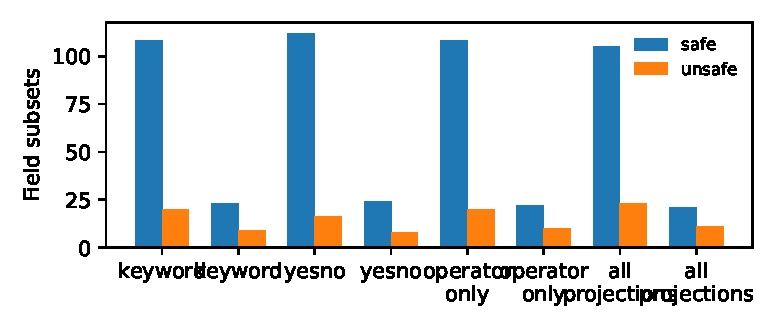
\includegraphics[width=\columnwidth]{figures/fig_semantic_frontier.pdf}
\caption{Semantic frontier over the core field lattice. Safe subsets repair all false equivalences in a scope; unsafe subsets retain a grounded counter-witness.}
\Description{A grouped bar chart comparing safe and unsafe field subsets for keyword, yes-no, operator-only, and all projections.}
\label{fig:semantic-frontier}
\end{figure}

\FloatBarrier

\section{Limitations and Conclusion}
\label{sec:conclusion}
OptSem-C is deliberately finite.  It audits a source-linked public-contract denominator, not private optimizer behavior, workload prevalence, or a population rate for database papers.  The current evidence chain is a single-extractor source-line protocol with replayable locators, digests, guards, paraphrases, downstream witnesses, and a recoding worksheet for independent follow-up; it does not claim inter-rater reliability.  DuckDB/PostgreSQL runs validate SQL constructability and visible-plan sanity for the generated denominator, not the truth of closed-source contracts.

Within that scope, the counted mechanisms are clear.  Placement separates local, delegated, distributed, and cloud execution; layer and decision time separate rewrite, planning, distribution, and runtime adaptation.  Across the 498 counted records, the ledger attributes differences to action variants (498), placement (466), layer (430), plan evidence (366), decision time (362), and operator family (281).  The practical workflow is short: name the coarse vocabulary, extract source-supported contracts, project them to the comparison table, and either retain the separating fields or state the intentionally coarse scope.  This is narrow but useful before latency or portability claims at federated SQL boundaries.
\FloatBarrier
